\section{Intressanta problem}
\subsection{Picking}
En av de sista sakerna jag implementerade var Picking så man kunde klicka på objekt i fönstret och välja filer och mappar. Jag trodde att detta skulle vara svårare men det var förvånansvärt lätt. Jag läste först om ett OpenGL hack där man renderar hela världen där varje objekt har olika färger och så kollar man vilken färg det är på pixeln som musen är på men detta verkade som ett rätt fult hack. Så istället så gjordes picking med hjälp av ray-casting. Jag fann väldigt mycket bra tips på denna hemsida \href{http://antongerdelan.net/opengl/raycasting.html}{Mouse Picking with Ray Casting}. 
\begin{center}
\begin{figure}[H]
    \centering
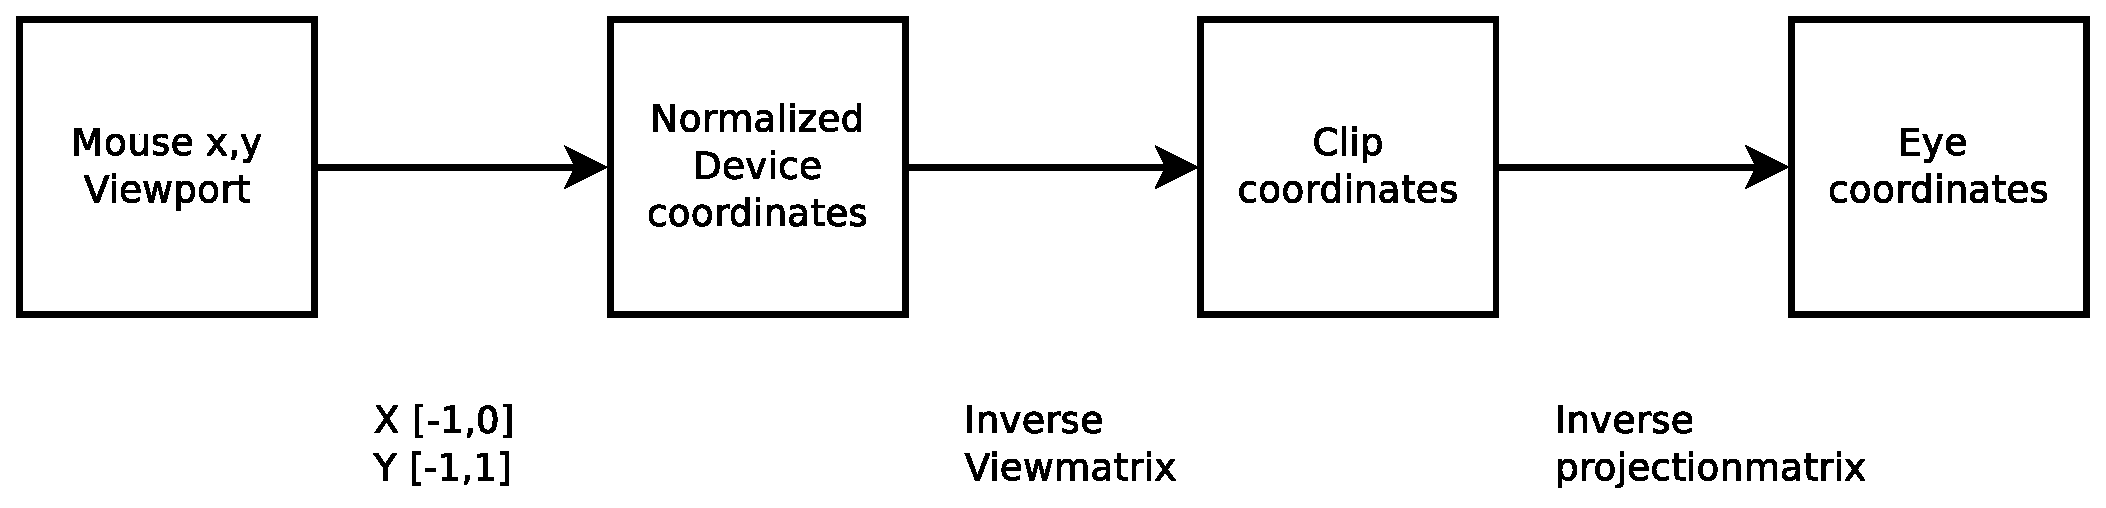
\includegraphics[width=8cm]{../grafik/picking.eps}
\caption{Picking.}
\label{fig:picking}
\end{figure}
\end{center}
Principen bakom picking med ray casting är helt enkelt att ta ett x och y värde på skärmen baklänges genom transformations pipelinen. 

\subsection{Texturer på alla bilder}
Alla filer som är bilder ska ha bilden som textur. Detta var lättare sagt än gjort. SOIL som är standarden vägrade fungera och CiMG gav bara svartvita bilder så till slut så valdes OpenCV för det är ett välbeprövat bibliotek som stödjer många filformat. De enda problemen med det var att OpenCV lagrar bilder från botten till toppen och OpenGL lagrar bilder från toppen till botten. Detta löstes genom att flippa bilden. Det andra problemet var ett OpenCV lagrar pixlar i BGR formatet men detta löstes med GL\_BGR som argument till glTexImage2D.

\subsection{Aliasing}
Något som syns väldigt tydligt i världen är aliasing då det är många kuber med skarpa kanter. Skulle jag fortsätta utveckla TMBTRF så skulle detta definitivt lösas med till exempel multisampling. 

\subsection{Text överläggning/regex}
Ett annat problem var att få upp en terminal ovanpå OpenGL. Detta löstes genom att använda X11 biblioteket och lägga på texten i fönstret efter att MicroGlut hade uppdaterat det. Detta gjorde att jag behövde få tillgång till fönsret och displayen samt skapa ett context för texten. Detta gjordes genom att modifiera MicroGlut. Jag ville också använda Regular expressions för att göra en så allmän terminal som möjligt men jag hade stora problem att få Regex att göra som jag ville. Den ansåg att fullständigt korrekta uttryck var fel så jag använde i slutändan rätt simpla uttryck kombinerat med tester om strängen från användaren innehöll en del ord för att välja rätt funktion.


